\chapter{Regression and Reconstruction on Cartesian Product Graphs} 

\label{chap:reg_and_rec} 

\lhead{Chapter 4. \emph{Regression and Reconstruction on Cartesian Product Graphs}} 


 
\section{Graph Products}

\label{sec:reg_and_rec_intro}

In this chapter, we turn our attention to the topic of signal processing on \textit{Cartesian product graphs}. This special class of graph finds applications in numerous areas, such as video, hyper-spectral image processing and network time series problems. However, the Cartesian product is not the only way to consistently define a product between two graphs. In this section we formally introduce the concept of a graph product, examine  some prominent examples, and explain why we choose to look specifically at the Cartesian graph product. 

\subsection{Basic definitions}

In the general case, consider two undirected graphs $\mathcal{G}_A = (\mathcal{V}_A, \mathcal{E}_A)$ and $\mathcal{G}_B = (\mathcal{V}_B, \mathcal{E}_B)$ with vertex sets given by $\mathcal{V}_A = \{a \in \mathbb{N} \, | \, a \leq A \}$ and $\mathcal{V}_B = \{b \in \mathbb{N} \, | \, b \leq B \}$ respectively. (In this context we do not regard zero to be an element of the natural numbers). A new graph $\mathcal{G}$ can be constructed by taking the product between $\mathcal{G}_A$ and $\mathcal{G}_B$. This can be generically written as follows. 

\begin{equation}
    \mathcal{G} = \mathcal{G}_A \, \diamond \, \mathcal{G}_B = (\mathcal{V}, \, \mathcal{E})
\end{equation}

For all definitions of a graph product, the new vertex set $\mathcal{V}$ is given by the Cartesian product of the vertex sets of the factor graphs, that is
 
\begin{equation}
    \mathcal{V} = \mathcal{V}_A \times \mathcal{V}_B = \{(a, \, b) \in \mathbb{N}^2 \, | \, a \leq A \; \text{and} \; b \leq B \}
\end{equation}


Typically, vertices are are arranged in lexicographic order, in the sense that $(a, \, b) \leq (a',\, b')$ iff $a < a'$ or ($a = a'$ and $b \leq b'$) \citep{Harzheim2005}. Each consistent rule for constructing the new edge set $\mathcal{E}$ corresponds to a different definition of a graph product. In general, there are eight possible conditions for deciding whether two nodes $(a, \, b)$ and $(a',\,  b')$ are to be connected in the new graph.

% visual? 


\begin{table}[h]
\def\arraystretch{1.5}
\centering
\begin{tabular}{lclc}
1. & $[a, \, a'] \in \mathcal{E}_A$ & and &  $b = b'$  \\
2. & $[a, \, a'] \notin \mathcal{E}_A$  & and &  $b = b'$  \\
3. & $[a, \, a'] \in \mathcal{E}_A$ & and &  $[b, \, b'] \in \mathcal{E}_B$ \\
4. & $[a, \, a'] \notin \mathcal{E}_A$ & and &  $[b, \, b'] \in \mathcal{E}_B$  \\
5. & $[a, \, a'] \in \mathcal{E}_A$ & and & $[b, \, b'] \notin \mathcal{E}_B$  \\
6. & $[a, \, a'] \notin \mathcal{E}_A$ & and & $[b, \, b'] \notin \mathcal{E}_B$  \\
7. & $a = a'$ & and & $[b, \, b'] \in \mathcal{E}_B$,  \\
8. & $a = a'$ & and &  $[b, \, b'] \notin \mathcal{E}_B$ 
\end{tabular}
\end{table}



Each definition of a graph product corresponds to the union of a specific subset of these conditions, thus, there exist 256 different types of graph product \citep{Barik2015}. Of these, the Cartesian product (conditions 1 or 7), the direct product (condition 3), the strong product (conditions 1, 3 or 7) and the lexicographic product (conditions 1, 3, 5 or 7) are referred to as the standard products and are well-studied \citep{Imrich2000}. A graphical depiction of the standard graph products is shown in figure \ref{fig:graph_products}. In each of these four cases, the adjacency and Laplacian matrices of the product graph can be described in terms of matrices relating to the factor graphs \citep{Fiedler1973, Barik2018}. This is shown in table \ref{tab:grap_product_matrices}. 

\begin{table}[h]
\def\arraystretch{1.8}
\centering
\small
\vspace{0.5cm}
\begin{tabular}{|l|cc|}
    \hline 

    & Adjacency matrix
    & Laplacian \\

    \hline

    Cartesian 
    & $\A_A \oplus \A_B$ 
    & $\LL_A \oplus \LL_B$ \\

    Direct 
    & $\A_A \otimes \A_B$  
    & $\D_A \otimes \LL_B + \LL_A \otimes \D_B - \LL_A \otimes \LL_B$ \\
    
    Strong 
    & $\A_A \otimes \A_B + \A_A \oplus \A_B$ 
    & $\D_A \otimes \LL_B + \LL_A \otimes \D_B - \LL_A \otimes \LL_B + \LL_A \oplus \LL_B$ \\

    Lexicographic 
    & $\I_A \otimes \A_B + \A_A \otimes \J_A$ 
    &  $\I_A \otimes \LL_B + \LL_A \otimes \J_B + \D_A \otimes (|\mathcal{V}_B| \I_B - \J_B)$ \\

    \hline

\end{tabular}
\vspace{0.2cm}
\caption[The adjacency and Laplacian matrices for the standard graph products]{The adjacency and Laplacian matrices for the standard graph products. Here, $\D_A$ and $\D_B$ are the diagonal degree matrices, i.e $\D_A = \diag{\A_A \mathbf{1}}$. $\I_A$ and $\J_A$ are the $(A \times A)$ identity matrix and matrix of ones respectively. } 
\vspace{0.3cm}
\label{tab:grap_product_matrices}
\end{table}

\begin{figure}[t]
    \begin{center}
    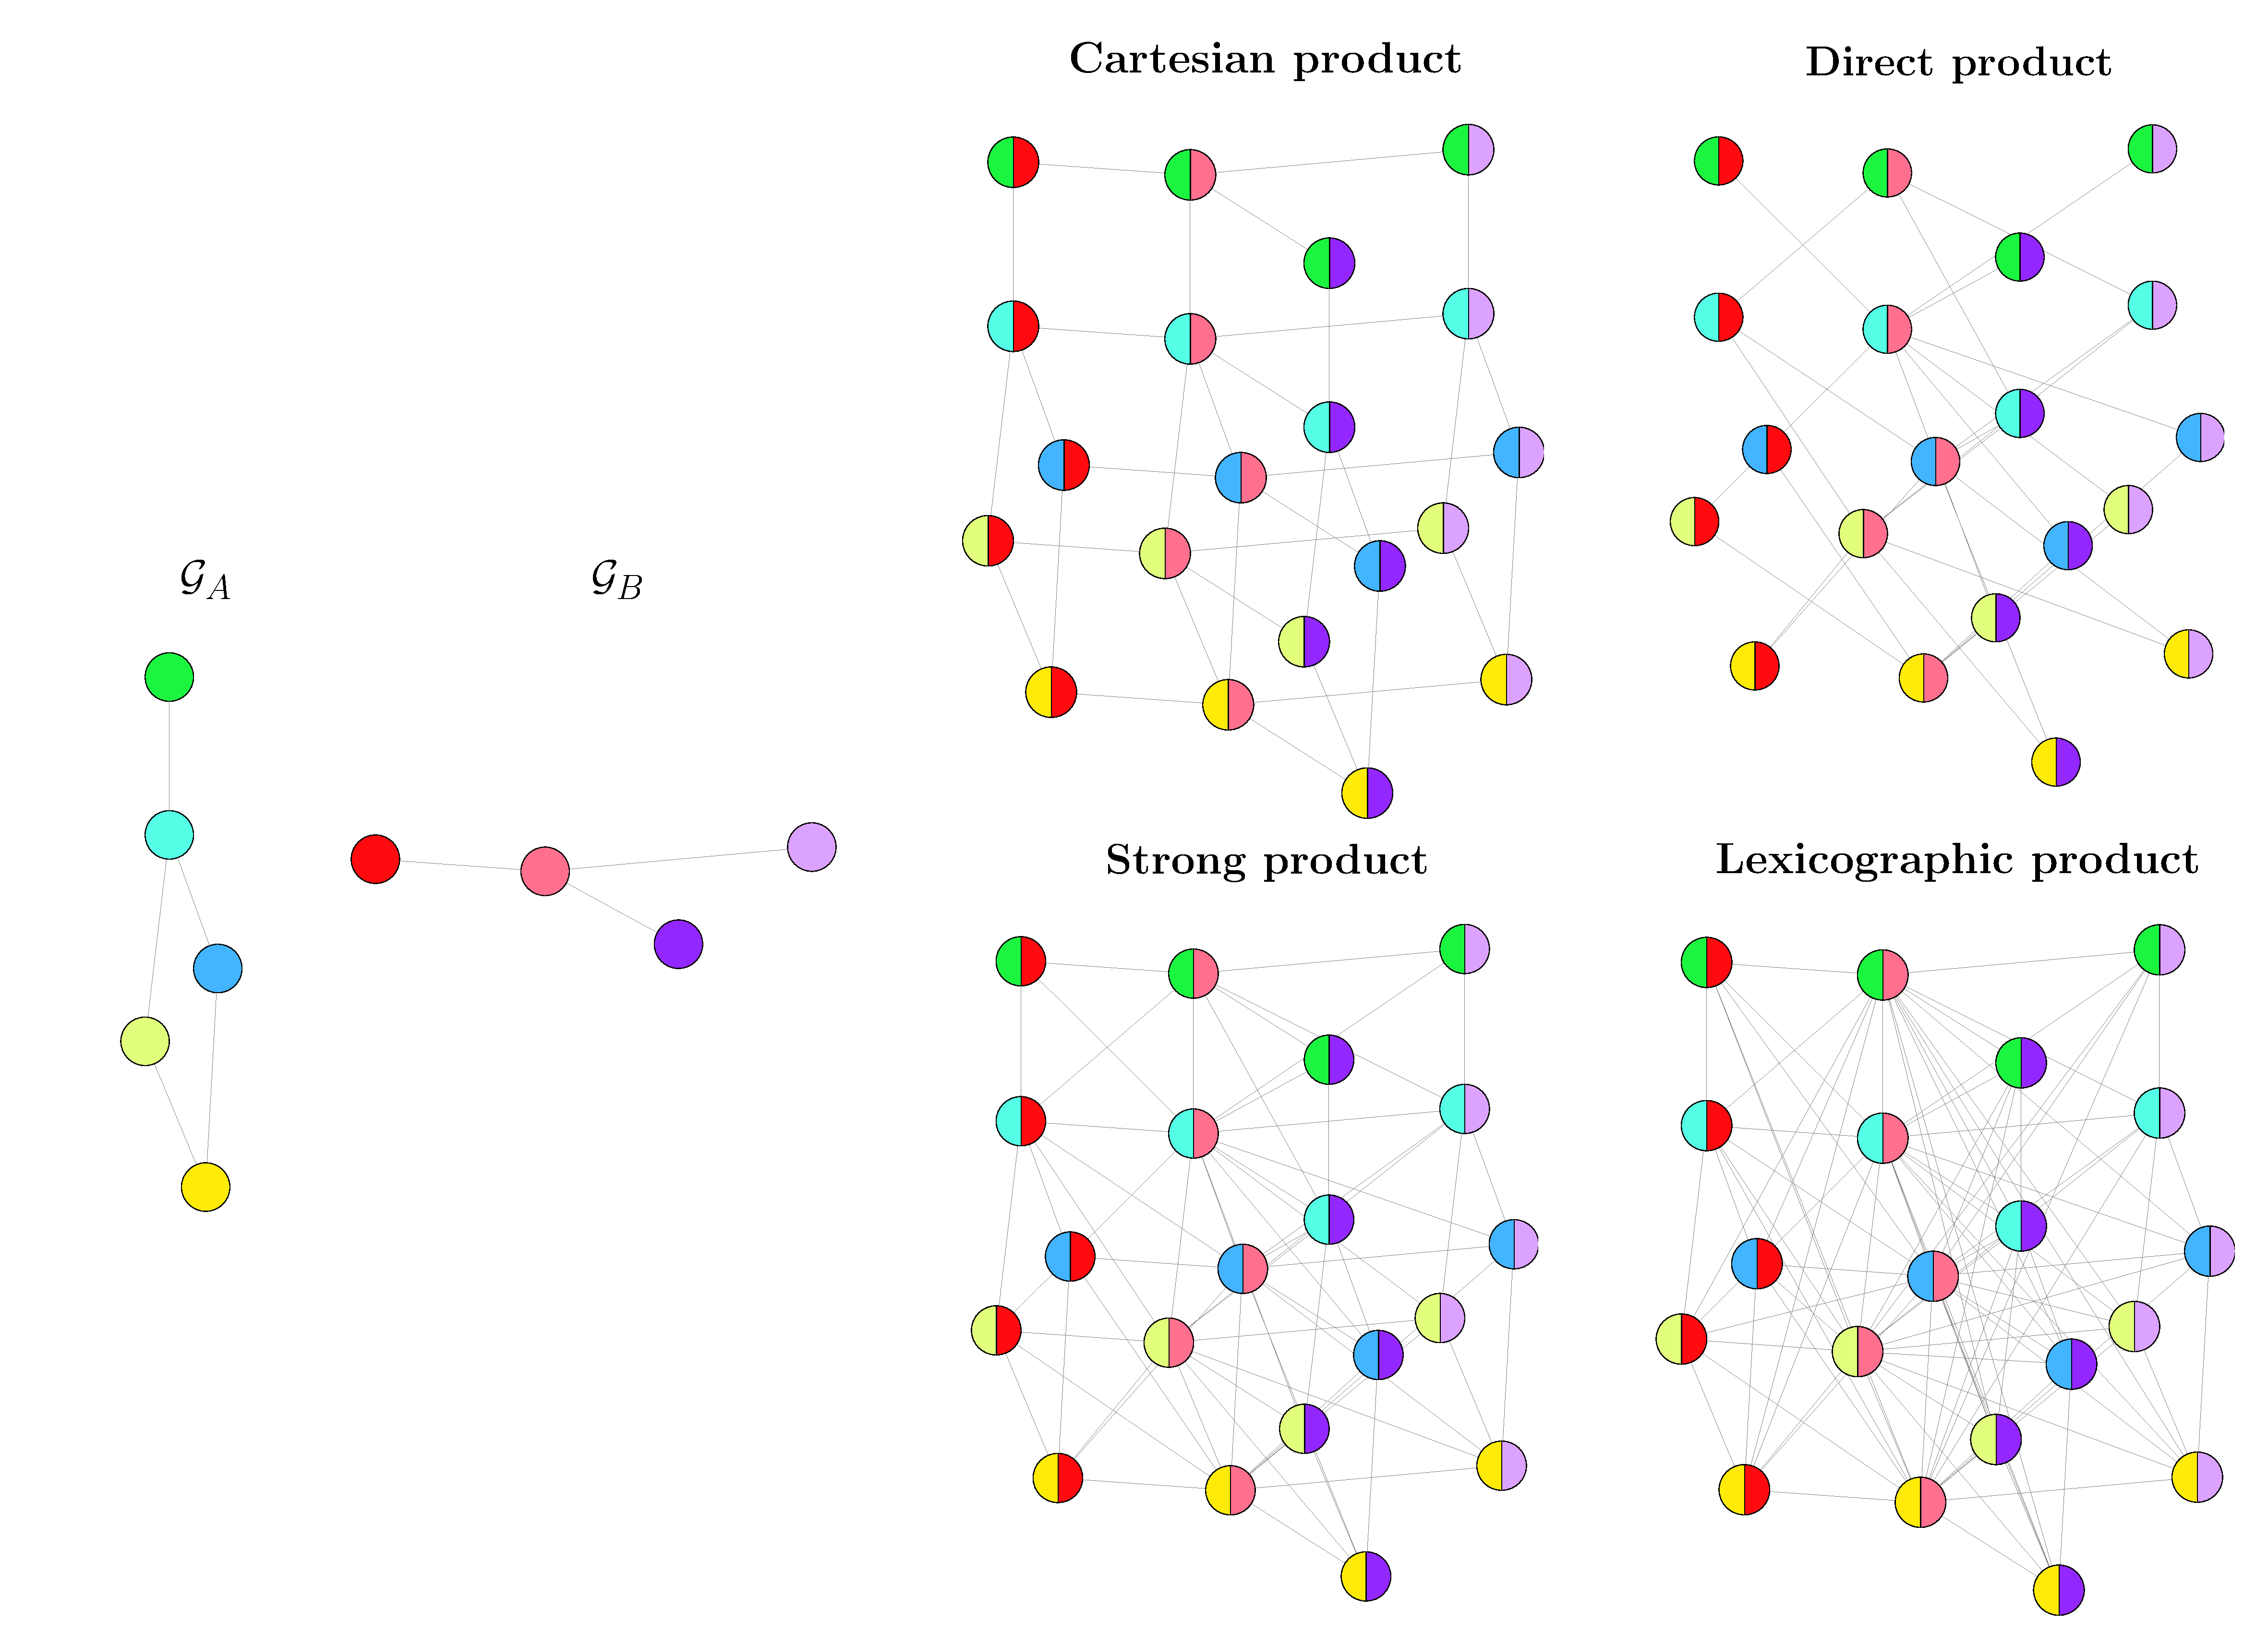
\includegraphics[width=\linewidth]{Figures/product_graphs.pdf}
    \end{center}
    \caption[Graphical depiction of the standard graph products]{A graphical depiction of the four standard graph products}
    \label{fig:graph_products}
\end{figure}

% choice of product effect the sparsity or A/cardinality of V

% What is the natural 256 ordering in terms of sparsity

% make small example in terms of vertex order

Given these definitions, it may seem that all the standard graph products are non-commutative in the sense that $\A_A \oplus \A_B  \neq \A_B \oplus \A_A $ etc. However, the graphs $\mathcal{G}_A \, \diamond \, \mathcal{G}_B$ and $\mathcal{G}_B \, \diamond \, \mathcal{G}_A$ are in fact isomorphically identical in the case of the Cartesian, direct and strong products. This is not the case for the Lexicographic product \citep{Imrich2000}. 

\subsection{The spectral properties of graph products}

In the field of graph signal processing, we are often concerned with analysing the properties of graphs via eigendecomposition of the graph Laplacian \citep{Mieghem2010}. In the case of product graphs, it is greatly preferable if we are able to fully describe the spectrum of $\mathcal{G}_A \diamond \mathcal{G}_B$ in terms of the spectra of $\mathcal{G}_A$ and $\mathcal{G}_B$ alone. This is because direct decomposition of a dense $\LL$ has time-complexity $O(A^3B^3)$, whereas decomposition of the factor Laplacians individually has complexity $O(A^3 + B^3)$. As the graphs under considerations become medium to large, this fact quickly makes direct decomposition of the product graph Laplacian intractable. However, in the general case, only the spectra of the Cartesian and lexicographic graph products can be described in this way \citep{Barik2018}. In the case of the direct and strong product, it is possible to estimate the spectra without performing the full decomposition (see \citep{Sayama2016}). However, in general, the full eigendecomposition of the product graph Laplacian can only be described in terms of the factor eigendecompositions when both factor graphs are regular. 


Consider the eigendecompositions of $\LL_A$ and $\LL_B$. 

\begin{equation}
    \LL_A = \U_A \LAM_A \U_A^\top, \aand \LL_B = \U_B \LAM_B \U_B^\top
\end{equation}

where $\U_A$ and $\U_B$ are the respective orthonormal eigenvector matrices, and $\LAM_A$ and $\LAM_B$ are the diagonal eigenvalue matrices given by 

\begin{equation}
    \LAM_A = \begin{bmatrix}
        \lambda_1^{(A)}, & & & \\
        & \lambda_2^{(A)} & & \\
        & & \ddots & \\
        & & & \lambda_A^{(A)} \\
    \end{bmatrix}  
    \aand 
    \LAM_B = \begin{bmatrix}
        \lambda_1^{(B)}, & & & \\
        & \lambda_2^{(B)} & & \\
        & & \ddots & \\
        & & & \lambda_B^{(B)} \\
    \end{bmatrix}  
\end{equation}

Given these definitions, table \ref{tab:product_graph_spectra} gives information about the spectral decomposition of the standard graph products.


\begin{table}[h]
    \def\arraystretch{1.8}
    \centering
    \small
    \vspace{0.5cm}
    \begin{tabular}{|l|cc|}
        \hline 
    
        & Eigenvalues
        & Eigenvectors \\
    
        \hline
    
        Cartesian 
        & $\lambda_a^{(A)} + \lambda_b^{(B)}$ 
        & $(\U_A)_a \otimes (\U_B)_b$ \\
    
        Direct$^{\star}$
        & $r_A \lambda_b^{(B)} + r_B \lambda_a^{(A)} - \lambda_a^{(A)} \lambda_b^{(B)}$  
        & $(\U_A)_a \otimes (\U_B)_b$ \\
        
        Strong$^{\star}$
        & $(1+r_A) \lambda_b^{(B)} + (1+r_B) \lambda_a ^{(A)}- \lambda_a^{(A)} \lambda_b^{(B)}$
        & $(\U_A)_a \otimes (\U_B)_b$ \\
    
        \multirow{2}{7em}{Lexicographic$^\dagger$}
        & $B \lambda_a^{(A)}$ 
        & $(\U_A)_a \otimes \mathbf{1}_B$ \\

        & $\lambda_b^{(B)} + B \text{deg}(a)$ 
        & $\mathbf{e}_a \otimes (\U_B)_b$  \\
    
        \hline
    
    \end{tabular}
    \vspace{0.2cm}
    \caption[Spectral decomposition of product graphs]{Eigendecomposition of the Laplacian of the standard graph products. Here, $a$ and $b$ are understood to run from 1 to $A$ and 1 to $B$ respectively. $\star$ only for $r_A$ and $r_B$-regular factor graphs. $\dagger$ note that the $b$ runs from 2 to $B$ in the lower row. } 
    \vspace{0.3cm}
    \label{tab:product_graph_spectra}
    \end{table}
    
% remark common degree locally only necessary 
% subspace concentration 


\subsection{GSP with Cartesian product graphs} 

While both the direct and strong products do find uses in certain applications (for example, see \citep{Kaveh2011}), they are both less common and more challenging to work with in a graph signal processing context due to their spectral properties described in the previous subsection. In practice, being limited to regular factor graphs means the majority of practical GSP applications are ruled out. The lexicographic product does not share this drawback, however it is also significantly less common than the Cartesian product in real-world applications. For this reason, in the following, we focus primarily on the Cartesian product. 

Given the spectral decomposition of the Cartesian graph product stated in table \ref{tab:product_graph_spectra}, we can write the Laplacian eigendecomposition in matrix form as follows. 

\begin{equation}
    \LL = \U \LAM \U^\top, \where \U = \U_A \otimes \U_B \aand \LAM = \LAM_A \oplus \LAM_B
\end{equation}

This motivates the following definitions for the Graph Fourier Transform (GFT) and its inverse (IGFT). Consider a signal defined over the nodes of a Cartesian product graph expressed as a matrix $\Y \in \R^{B \times A}$. We can perform the GFT as follows. 

\begin{equation}
    \text{GFT}(\Y) = \MAT{\big( \U_A^\top \otimes \U_B^\top \big) \, \vecc{\Y}} = \U_B^\top \F \U_A
\end{equation}

Correspondingly, we can define the IGFT acting on a matrix of spectral components $\Z \in \R^{B \times A}$ as follows. 

\begin{equation}
    \text{IGFT}(\Z) = \MAT{\big( \U_A \otimes \U_B \big)\,\vecc{\Y}} = \U_B \Z \U_A^\top
\end{equation}


\note{Product graph signals: repseprentation and vectorisation}{

    It is natural to assume that signals defined on the nodes of a Cartesian product graph $\mathcal{G}_A \, \square \; \mathcal{G}_B$ could be represented by matrices (order two tensors) of shape $(A \times B)$. Since product graph operators, such as the Laplacian $\LL_A \oplus \LL_B$, act on vectors of length $AB$, we must define a consistent function to map matrix graph signals $\in \R^{A \times B}$ to vector graph signals $\in \R^{AB}$. The standard mathematical operator for this purpose is the $\vecc{\cdot}$ function, along with its reverse operator $\mat{\cdot}$. However, this is somewhat problematic since $\vecc{\cdot}$ is defined to act in \textit{column-major} order, that is 

    $$
    \text{vec} \left( \begin{bmatrix}
        \Y_{(1, 1)} & \Y_{(1, 2)} & \dots & \Y_{(1, B)} \\
        \Y_{(2, 1)} & \Y_{(2, 2)} & \dots  & \Y_{(2, B)} \\
        \vdots & \vdots & \ddots & \vdots \\
        \Y_{(A, 1)} & \Y_{(A, 2)} & \dots  & \Y_{(A, B)} \\
    \end{bmatrix} \right) 
    =
    \begin{bmatrix}
        \Y_{(1, 1)} \\ \Y_{(2, 1)} \\ \vdots \\ \Y_{(A-1, B)} \\ \Y_{(A, B)}
    \end{bmatrix}
    $$

    As is visible, this does not result in a lexicographic ordering of the matrix elements when the graph signal has shape $(A \times B)$. Therefore, to avoid this issue and to be consistent with standard mathematical notation, we will assume that graph signals are represented by matrices  of shape $(B \times A)$ when considering the product between two graphs $\mathcal{G}_A \, \square \, \mathcal{G}_B$. For graph signals of this shape, the first index represents traversal of the nodes in $\mathcal{G}_B$, and the second index represents traversal of the nodes in $\mathcal{G}_A$. This ensures that matrix elements are correctly mapped to vector elements when using the column-major $\vecc{\cdot}$ function. 

}

Given these definitions, we can define a spectral operator (usually a low-pass filter) $\HH$ which acts on graph signals according to a spectral scaling function $g(\lambda \,; \, \beta)$ such as one of those defined in table \ref{tab:iso_filters}. As with regular non-product graphs, the action of this operator can be understood as first transforming a signal into the frequency domain via the GFT, then scaling the spectral components according to some function, and finally transforming back into the vertex domain via the IGFT. 

\begin{align} 
    \label{eq:graph_filter}
    \HH &= g(\LL_A \oplus \LL_B) \notag \\ 
       &= \big( \U_A \otimes \U_B \big) \, g \big( \LAM_A \oplus \LAM_B \big) \, \big( \U_A^\top \otimes \U_B^\top \big) \notag \\
       &= \big( \U_A \otimes \U_B \big) \, \Diag{\vecc{\G}} \, \big( \U_A^\top \otimes \U_B^\top \big)
\end{align}

The matrix $\G \in \R^{B \times A}$, which we refer to as the spectral scaling matrix, holds the value of the scaling function applied to the sum of
pairs of eigenvalues, such that

\begin{equation}
    \G_{ba} = g(\lambda^{(A)}_a + \lambda^{(B)}_b; \beta)
\end{equation}

We observe that defining the filtering operation in this manner implies that the intensity is equal across both $\mathcal{G}_A$ and $\mathcal{G}_B$. We refer to filters of this type as \textit{isotropic}. This can be further generalised by considering an \textit{anisotropic} graph filter, which offers independent control over the filter intensity in each of the two dimensions. In this case, we define $\G$ as follows. 

\begin{equation}
    \G_{ba} =  g \left( \begin{bmatrix}
        \lambda^{(A)}_a \\ \lambda^{(B)}_b 
    \end{bmatrix}, \; \begin{bmatrix}
        \beta_a \\ \beta_b 
    \end{bmatrix} \right)
\end{equation}

where now $g(\lambdaa \,; \, \betaa)$ is chosen to be an anisotropic graph filter such as one of those listed in table \ref{tab:anis_filters}. Note that the original parameter $\beta$ is now replaced by a vector of parameters $\betaa$ which control the filter intensity in each dimension. 

\begin{table}[t]
    \def\arraystretch{1.7}
    \small
    \begin{center}
    \begin{tabular}{|l|c|}
    \hline
    \textbf{Filter}   & $g(\lambdaa; \,\betaa)$    \\ 
    \hline
    1-hop random walk & $(1 + \betaa^\top\lambdaa)^{-1}$ \\
    \hline
    Diffusion         & $\exp(-\betaa^\top\lambdaa)$       \\
    \hline
    ReLu              & $\max (1 - \betaa^\top\lambdaa, 0)$  \\
    \hline
    Sigmoid           & $2 \big( 1 + \exp(\betaa^\top\lambdaa)\big)^{-1}$ \\
    \hline
    Bandlimited       & $1, \,\text{if} \; \betaa^\top\lambdaa \leq 1 \; \text{else} \; 0$   \\
    \hline
    \end{tabular}
    \end{center}
    \caption{Anisotropic graph filter functions}
    \label{tab:anis_filters}
    \end{table}



\section{Graph Signal Reconstruction on Cartesian Product Graphs}

\label{sec:gsr_cpg}

We now turn our attention to the task of signal reconstruction on Cartesian product graphs. In the following, we will replace the factor graph labels $A$ and $B$ with $T$ and $N$ respectively. The reason for this is that one application of particular interest is graph time-series problems, where we seek to model a network of $N$ nodes across a series of $T$ discrete time points. These so called ``time-vertex'' (T-V) problems have garnered significant interest recently in the context of GSP \citep{Grassi2018, Isufi2017, Loukas2016}. T-V signals can be understood as existing on the nodes of a Cartesian product graph $\mathcal{G}_T \, \square \, \mathcal{G}_N$. In particular, we can conceptualise $T$ repeated measurements of a signal defined across the nodes of a $N$-node graph as a single measurement of a signal defined on the nodes of $\mathcal{G}_T \, \square \, \mathcal{G}_N$, where $\mathcal{G}_T$ is a simple path graph.

\vspace{1cm}


\begin{figure}[b]
    \begin{center}
    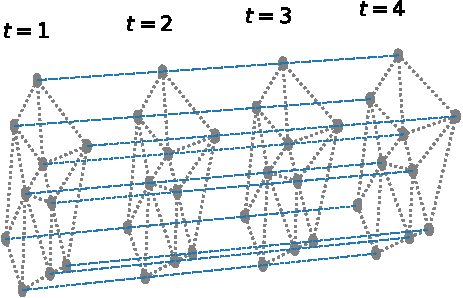
\includegraphics[width=0.5\linewidth]{Figures/T-V.pdf}
    \end{center}
    \caption[A time-vertex Cartesian product graph]{A graphical depiction of a time-vertex Cartesian product graph}
    \label{fig:TV}
\end{figure}



\note{On the Laplacian spectrum of the path graph}{
    When considering time-vertex problems, $\mathcal{G}_T$ will generally be described by a  path graph. This special case of a graph has vertices given by $\mathcal{V}_T = \{t \in \mathbb{N} \, | \, t \leq T \}$ and edges given by $\mathcal{E}_T = \{ \, [t, t+1] \, | \, t < T \}$. The Laplacian matrix of the path graph is therefore given by 

    $$
    \LL_T = \begin{bmatrix}
        1 & -1 & & & \\
        -1 & 2 & -1 & &   \\
        & & \ddots & &   \\
        & &  -1 & 2 & -1 \\
        & & &  -1 & 1 \\
    \end{bmatrix}
    $$

    The eigenvalues and eigenvectors of this Laplacian are well-known and can be expressed in closed-form \citep{Jiang2012}. In particular, 

    $$
    \lambda^{(T)}_t = 2 - 2 \cos \Big(  \, \frac{t - 1}{T} \pi \, \Big)
    $$

    and 

    $$
    (\U_T)_{ij} = \cos \Big( \, \frac{j - 1}{T}\big(i - 0.5\big)\pi \, \Big)
    $$

    ($\U_T$ should be appropriately normalised after this computation to ensure each column is orthonormal). Computing the eigendecomposition directly in this fashion reduces the complexity from $O(T^3)$ to $O(T^2)$ which can be significant for large time-series problems. 
 
}

Note that, despite the observation that $\mathcal{G}_T$ is often a path graph in the context of T-V problems, the methods introduced in this section are valid for the Cartesian product between arbitrary undirected factor graphs. 

\subsection{Problem statement}


The goal of Graph Signal Reconstruction (GSR) is to estimate the value of a partially observed graph signal at nodes where no data was collected. In the context of GSR on a Cartesian product graph, the available data is an observed signal $\Y \in \R^{N \times T}$ where only a partial set $\mathcal{S} = \{(n_1, t_1), (n_2, t_2), \dots \}$ of the signal elements were recorded. All other missing elements of $\Y$ are set to zero. Our model is based on the assumption that $\Y$ is a noisy partial observation of an underlying signal $\F \in \R^{N \times T}$, which is itself assumed to be smooth with respect to the graph topology. 

We define the statistical model for the generation of an observation matrix $\Y$ as 

\begin{equation}
    \Y = \Ss \circ \big(\F + \E \big)
\end{equation}

where $\Ss \in [0, 1]^{N \times T}$ is referred to as the sensing matrix, and has entries given by 

\begin{equation}
    \Ss_{nt} = \begin{cases}
        1 & \text{if} \;\; (n, t) \in \mathcal{S} \\
        0 & \text{otherwise}
    \end{cases}
\end{equation}

The matrix $\E$ represents the model error and is assumed to have an independent normal distribution with unit variance. Therefore, the probability distribution of $\Y$ given the latent signal $\F$ is

\begin{equation}
    \label{eq:Y_given_F}
    \vecc{\Y} \, | \, \F \sim \mathcal{N}\Big(\vecc{\Ss \circ \F}, \; \Diag{\vecc{\Ss}}\Big)
\end{equation}

Note that the covariance matrix $\Diag{\vecc{\Ss}}$ is semi-positive definite by construction. This naturally reflects the constraint that some elements of $\Y$ are zero with probability 1. In order to estimate the latent signal $\F$, we must provide a prior distribution describing our belief about its likely profile ahead of time. In general, we expect $\F$ to be smooth with respect to the topology of the graph. This can be expressed by setting the covariance matrix in its prior to be proportional to $\HH^2$, where $\HH$ is a graph filter as defined in equation (\ref{eq:graph_filter}). For now, in the absence of any further information, we assume that the prior mean for $\F$ is zero across all elements. 

\begin{equation}
    \vecc{\F} \sim \mathcal{N}\big(\mathbf{0}, \, \gamma^{-1} \HH^2\big) 
\end{equation}

Next, given an observation $\Y$, we use Bayes' rule to find the posterior distribution over $\F$. This is given by

\begin{equation}
    \pi\big(\vecc{\F} \, | \, \Y \big) = \frac{\pi\big(\vecc{\Y} \, | \, \F \big) \pi(\F) }{\pi(\Y)}.
\end{equation}

where we use the notation $\pi(\cdot)$ to denote a probability density function.

\begin{theorem}
    The posterior distribution for $\F$ is given by 

    \begin{equation}
        \label{eq:F_post}
            \Vecc{\F} \, | \, \Y \sim \mathcal{N} \big(\SIG \, \Vecc{\Y}, \; \SIG \big)
        \end{equation}
        
        \noindent where 
        
        \begin{equation}
        \label{eq:Sig_post}
            \SIG = \Big(\Diag{\vecc{\Ss}} + \gamma  \HH^{-2}\Big)^{-1}
        \end{equation}

\end{theorem}

\begin{proof}
    Consider the matrix $\Ss_{\epsilon}$ defined in the following manner. 
    
    \begin{equation}
        (\Ss_{\epsilon})_{nt} = \begin{cases}
            1 & \text{if} \;\; (n, t) \in \mathcal{S} \\
            \epsilon & \text{otherwise}
        \end{cases}
    \end{equation}

    We can use this definition to rewrite equation \ref{eq:Y_given_F} for the probability distribution of $\Y | \F$.

    \begin{equation}
        \Vecc{\Y} \, | \, \F \, \sim \, \lim_{\epsilon \rightarrow 0} \, \Bigg[ \, \mathcal{N}\Big(\vecc{\Ss_{\epsilon} \circ \F}, \; \Diag{\vecc{\Ss_{\epsilon}}}\Big) \, \Bigg]
    \end{equation}

    In this way, the negative log-likelihood of an observation $\Y | \F$ is given by 

    \begin{equation}
        \label{eq:log_prob_1}
        - \log \pi(\Y | \F) = \lim_{\epsilon \rightarrow 0} \, \Bigg[  \frac{1}{2} \vecc{\Ss_{\epsilon} \circ \F - \Y}^\top \Diag{\vecc{\Ss_{\epsilon}}}^{-1} \vecc{\Ss_{\epsilon} \circ \F - \Y}\, \Bigg]
    \end{equation}

    up to an additive constant which does not depend on $\F$. Note that, since $\Y = \Ss_{\epsilon}  \circ \Y$, we can rewrite $\vecc{\Ss_{\epsilon} \circ \F - \Y}$ as 

    \begin{align}
        \vecc{\Ss_{\epsilon} \circ \F - \Y} &= \Vecc{\Ss_{\epsilon} \circ  (\F - \Y)}  \notag \\
        &= \Diag{\vecc{\Ss_{\epsilon}}} \vecc{\F - \Y}
    \end{align}

    Therefore, equation \ref{eq:log_prob_1} can be rewritten as 

    \begin{align}
        - \log \pi(\Y | \F) &= \lim_{\epsilon \rightarrow 0} \, \Bigg[  \frac{1}{2} \vecc{\F - \Y}^\top \Diag{\vecc{\Ss_{\epsilon}}} \, \vecc{\F - \Y}\, \Bigg] \notag \\[0.2cm]
        &= \frac{1}{2} \vecc{\F - \Y}^\top \Diag{\vecc{\Ss}} \, \vecc{\F - \Y}
    \end{align}

    Now consider the full log-posterior. Using Bayes rule, this can be written as 

    \begin{multline}
        -\log \pi\big(\vecc{\F} \, | \, \Y \big) = \frac{1}{2} \vecc{\F - \Y}^\top \Diag{\vecc{\Ss}} \, \vecc{\F - \Y} \; + \\ \frac{\gamma}{2} \vecc{\F }^\top\HH^{-2} \, \vecc{\F}
    \end{multline}

    Up to an additive constant not dependent $\F$, this can be written as 

    \begin{equation}
        -\log \pi\big(\vecc{\F} \, | \, \Y \big) = \frac{1}{2} \Big( \vecc{\F}^\top \big( \Diag{\vecc{\Ss}} + \gamma \HH^{-2}\big) \vecc{\F} - 2 \, \vecc{\Y}^\top \F \Big)
    \end{equation}

    Using the conjugacy of the normal distribution, by direct inspection we can conclude that the posterior covariance is given by 

    \begin{equation}
        \SIG = \Big( \Diag{\vecc{\Ss}} + \gamma \HH^{-2} \Big)^{-1}
    \end{equation}

    and that the posterior mean is given by $\SIG \, \vecc{\Y}$. 

\end{proof}

In this chapter, we are primarily interested in computing the posterior mean, which is the solution to the following linear system. 

\begin{equation}
    \label{eq:lin_system}
        \Big(\Diag{\vecc{\Ss}} + \gamma  \HH^{-2}\Big) \, \vecc{\F} = \vecc{\Y}
    \end{equation}

We return to the question of sampling and estimating the posterior covariance in chapter \ref{chap:variance}. 


\subsection{A stationary iterative method}

Hello

\subsection{A conjugate gradient method}

Hello

\subsection{Convergence properties}

Hello

\subsection{Image processing experiments}

Hello



\section{Kernel Graph Regression with Unrestricted Missing Data Patterns}

\label{sec:kgr_mdp}

Hello

\subsection{Cartesian product graphs and KGR}

Hello

\subsection{Convergence properties}

Hello


\section{Regression with Network Cohesion}

\label{sec:rnc_mdp}

Hello

\subsection{Regression with node-level covariates}

Hello

\subsection{Convergence properties}

Hello


\section{Multi-Dimensional Cartesian Product Graphs}

\label{sec:nd_gsp}

Hello

\subsection{Fast computation with \textit{d}-dimensional Kronecker products}

Hello

\subsection{Signal reconstruction}

Hello

\subsection{Kernel Graph Regression}

Hello

\subsection{Regression with Network Cohesion}


